% vim: set foldmethod=marker foldlevel=0:

\documentclass[a4paper]{article}
\usepackage[UKenglish]{babel}

% NOTE: hyperref has to come before preamble
\usepackage{hyperref}

\usepackage{preamble}

\usepackage{graphicx}
\graphicspath{ {./imgs/} }

\title{MA144 Methods of Mathematical Modelling 2, Assignment 1}
\author{Dyson Dyson}
\date{}

\begin{document}

\maketitle

\setlength{\parindent}{0em}
\setlength{\parskip}{1em}

% {{{ Q1
\question{1}

\subsection{~}

The polar curve with equation $r = f(\theta)$ can be parametrised as $\ul r (\theta) = (f(\theta) \cos \theta, f(\theta) \sin \theta)$. Then $$\dd{\ul r}\theta = \l(\dd f\theta (\theta) \cos \theta - f(\theta) \sin \theta, \dd f\theta (\theta) \sin \theta + f(\theta) \cos \theta\r)$$
Therefore \begin{align*}
\| \ul r\,'(\theta) \| &= \sqrt{\l( f'(\theta) \cos \theta - f(\theta) \sin \theta \r)^2 + \l( f'(\theta) \sin \theta + f(\theta) \cos \theta \r)^2}\\[1ex]
&= \sqrt{f'(\theta)^2 \cos^2 \theta - 2 f(\theta) f'(\theta) \cos\theta \sin\theta + f(\theta)^2 \sin^2 \theta}\\[1ex]
&\phantom{=} \overline{+ f'(\theta)^2 \sin^2 + 2 f(\theta) f'(\theta) \cos\theta \sin\theta + f(\theta)^2 \cos^2 \theta}\\[1ex]
&= \sqrt{f'(\theta)^2 (\cos^2 \theta + \sin^2 \theta) + f(\theta)^2 (\cos^2 \theta + \sin^2 \theta)}\\[1ex]
&= \sqrt{f'(\theta)^2 + f(\theta)^2}\\[1ex]
&= \sqrt{\l(\dd f\theta\r)^2 + f^2}\\[1ex]
\end{align*}

Therefore the arc length of the curve is $$s = \intlim ab {\sqrt{\l(\dd f\theta\r)^2 + f^2}}\theta$$ as required.

\subsection{~}

Let $r = 1 + \cos\theta$. %Then $\ul r(\theta) = (\cos\theta + \cos^2\theta, \sin\theta + \sin\theta\cos\theta)$.

\begin{figure}[h]
	\centering
	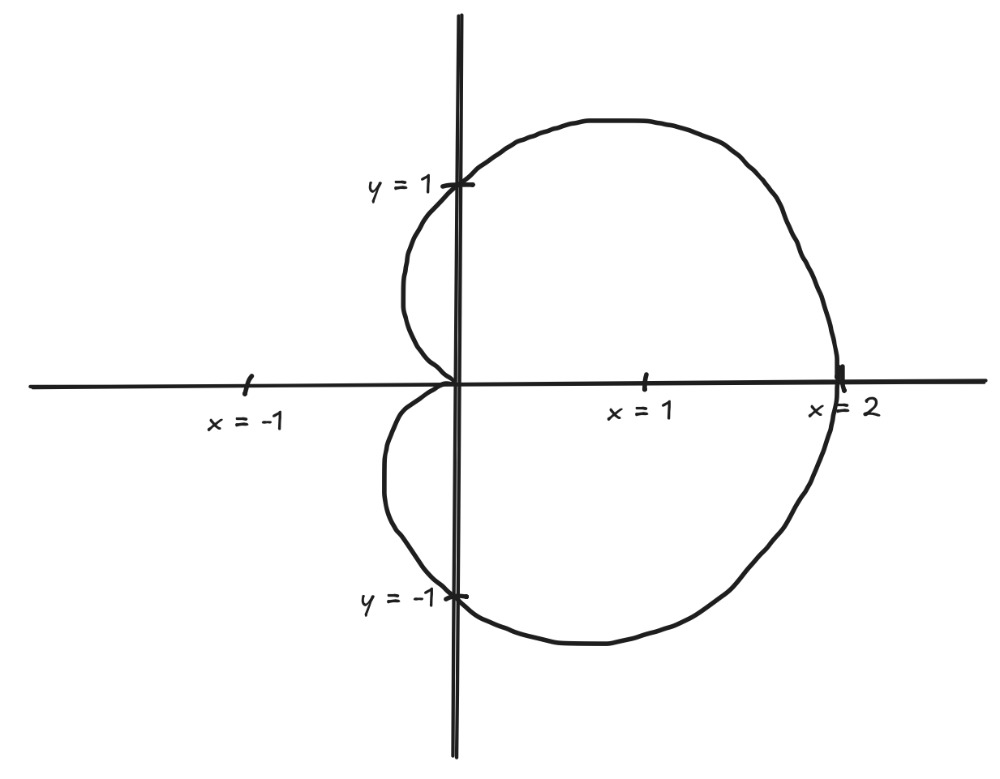
\includegraphics[scale=0.3]{Q1b}
	\caption{A sketch of $r = 1 + \cos\theta$}
\end{figure}

$\ds\dd r\theta = -\sin\theta$ so the arc length is \begin{align*}
s &= \intlim 0{2\pi} {\sqrt{\sin^2 \theta + (1 + \cos\theta)^2}} \theta\\[1ex]
&= \intlim 0{2\pi} {\sqrt{\sin^2 \theta + 1 + 2\cos\theta + \cos^2 \theta}} \theta\\[1ex]
&= \intlim 0{2\pi} {\sqrt{2 + 2\cos\theta}} \theta
\end{align*}
I don't know how to do this integral but apparently it's $4\pi$.

\subsection{~}

% TODO: Justify this
The curve given by $r = 1 + \cos k\theta$ is non-simple whenever $k$ is not an integer.
% }}}

% {{{ Q2
\question{2}

Consider the curve $\cal C$ with equation $$\quad 4y^2 - 9x^2 = 1, \quad y > 0$$

\subsection{~}

Since $\cosh^2 t - \sinh^2 t = 1$, we can let $y = \f12 \cosh t$ and $x = \f13 \sinh t$. Then we'll have the equation of $\cal C$. Therefore we can parametrise $\cal C$ as $\ul r(t) = \l( \f13 \sinh t, \f12 \cosh t \r)$.

Since $\f12 \cosh t > 0$ for all $t \in (-\infty, \infty)$, the requirement of $y>0$ is satisfied by $t \in (-\infty, \infty)$, so that's the range of this parametrisation.

\subsection{~}

\begin{figure}[h]
	\centering
	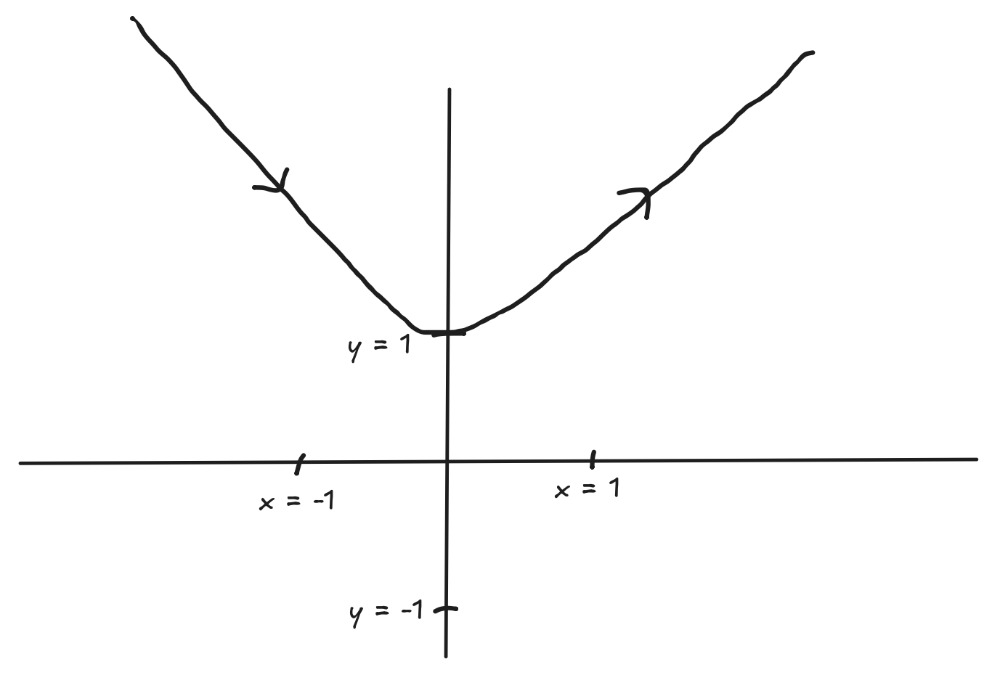
\includegraphics[scale=0.3]{Q2b}
	\caption{A sketch of $\ul r(t) = \l( \f13 \sinh t, \f12 \cosh t \r)$}
\end{figure}

There is a turning point at $\l(0, \f12\r)$ and asymptotes are $y = \f32 x$ and $y = -\f32 x$.

\subsection{~}

% TODO: Reparametrise with $u$ such that $0 < u < 1$
% }}}

% {{{ Q3
\question{3}

\subsection{~}

\begin{figure}[h]
	\centering
	\begin{tabular}{cc}
		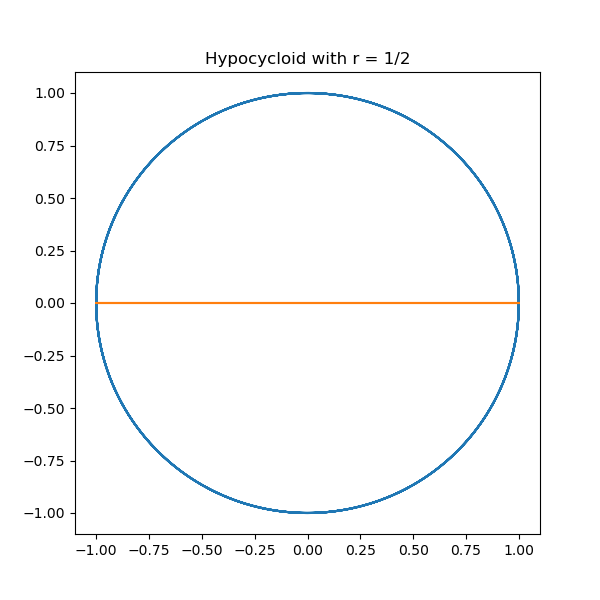
\includegraphics[scale=0.4]{Q3a-1} & 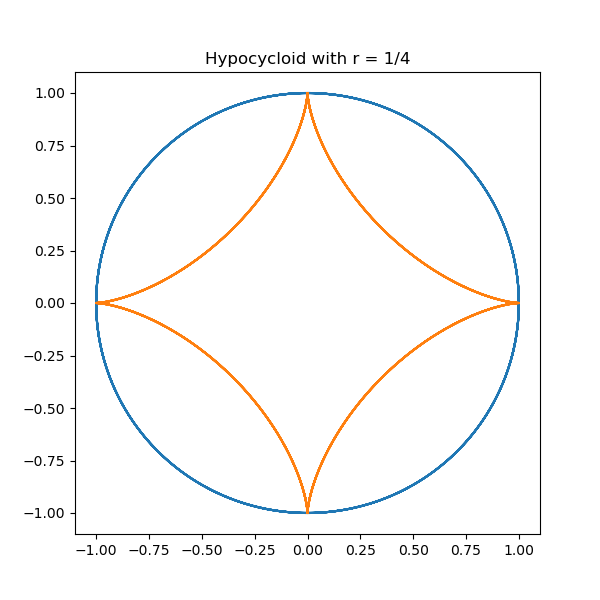
\includegraphics[scale=0.4]{Q3a-2}\\
		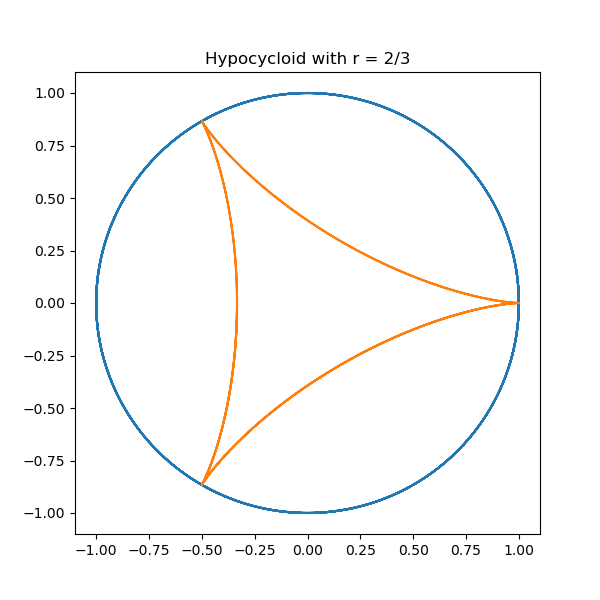
\includegraphics[scale=0.4]{Q3a-3} & 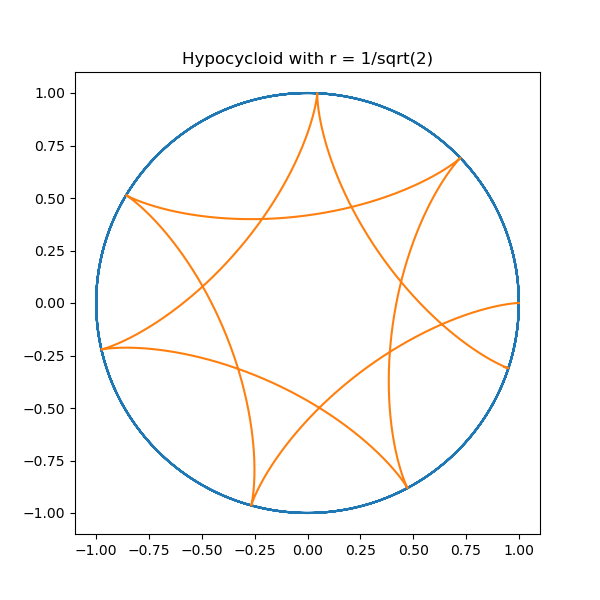
\includegraphics[scale=0.4]{Q3a-4}
	\end{tabular}
	\caption{Plots of hypocycloids for various values of $r$}
	\label{fig:hypocycloid-plots}
\end{figure}

\begin{figure}[h]
	\centering
	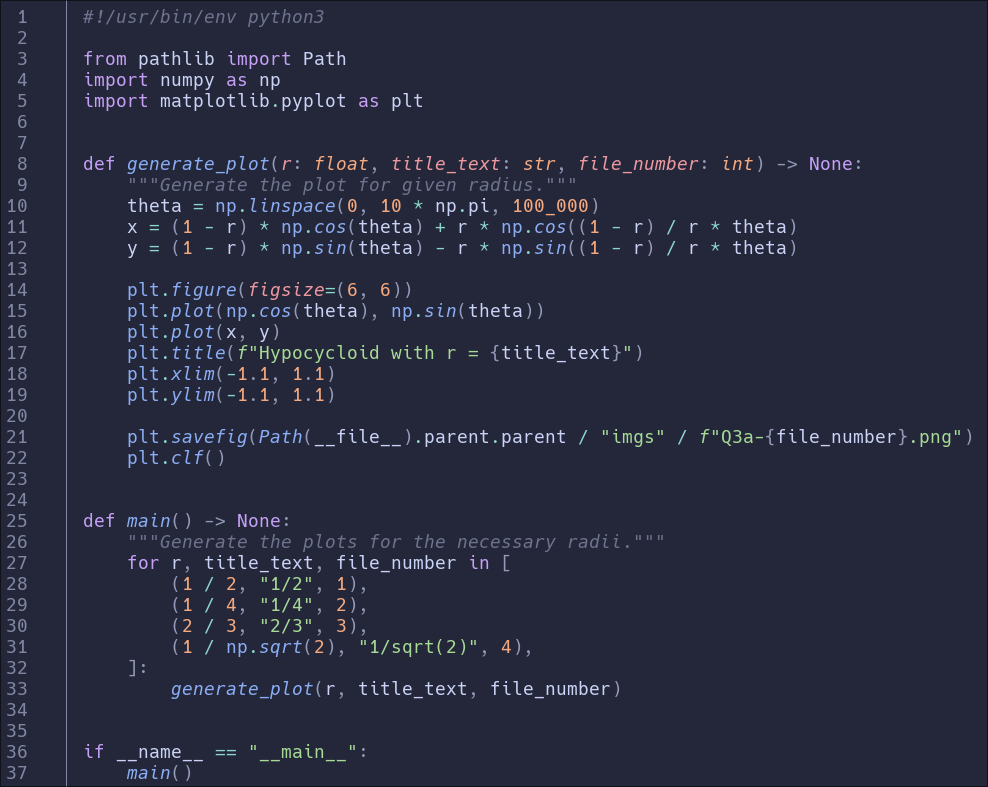
\includegraphics[scale=0.3]{Q3a-code}
	\caption{The code used to generate the plots in Figure~\ref{fig:hypocycloid-plots}. The code can also be found \href{https://github.com/DoctorDalek1963/uni/blob/fe244f6880c7df0d801d426ca7ef9149b585ec2f/first-year/MA144-Methods-of-Mathematical-Modelling-2/Ass 1/code/generate_plots.py}{on GitHub}}
\end{figure}

\subsection{~}

I conjecture that for any $r \in \R$, the curve will be closed if and only if $r \in \Q$.
% }}}

\end{document}
